\section*{Appendix -- BayesDAG: Gradient-Based Posterior Sampling for Causal Discovery}
\section{Joint Inference with SG-MCMC}
\label{appsec: joint inference SG-MCMC}
\begin{wrapfigure}[12]{r}{0.4\textwidth}
   \usetikzlibrary{bayesnet}
\scalebox{0.7}{
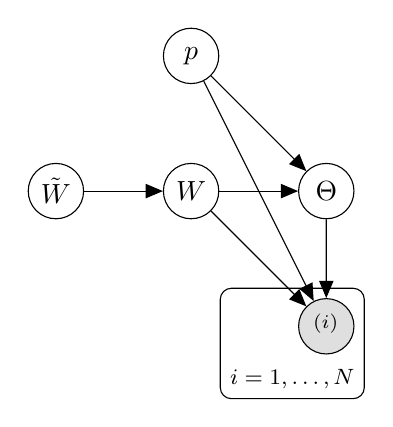
\begin{tikzpicture}[scale=3]

  % Define nodes
  \node[latent] (Wtilde) {$\tilde{W}$};
  \node[latent, right=of Wtilde] (W) {$W$};
  \node[latent, above=of W] (p) {$p$};
  \node[latent, right=of W] (Theta) {$\Theta$};
  \node[obs, below=of Theta] (x) {$\vx^{(i)}$};
  
  % Connect nodes
  \edge {Wtilde} {W};
  \edge {p} {x};
  \edge {W} {Theta};
  \edge {W} {x};
  \edge {Theta} {x};
  \edge {p} {Theta};
  
  % Define plate
  \plate {x_plate} {(x)} {$i = 1, \dots, N$};

\end{tikzpicture}
}
   \caption{Graphical model with latent variable $\tmW$.}
   \label{fig: graphical model with latent}
\end{wrapfigure}

In this section, we propose an alternative formulation that enables a joint inference framework for $\vp,\mW,\mTheta$ using SG-MCMC, thereby avoiding the need for variational inference for $\mW$.

We adopt a continuous relaxation of $\mW$, similar to \cite{lorch2021dibs}, by introducing a latent variable $\tmW$. The graphical model is illustrated in \cref{fig: graphical model with latent}.  We can define 
\begin{equation}
   p(\mW|\tmW) = \prod_{i,j} p(W_{ij}|\tilde{W}_{ij})
   \label{eq: W and tilde W forward prob}
\end{equation}
with $p(W_{ij}=1|\tilde{W}_{ij})=\sigma(\tilde{W}_{ij})$ where $\sigma(\cdot)$ is the sigmoid function. In other words, $\tilde{W}{ij}$ defines the existence logits of $W{ij}$.

With the introduction of $\tmW$, the original posterior expectations of $p(\vp,\mW,\mTheta\vert \mD)$, e.g.~during evaluation, can be translated using the following proposition. 
\begin{proposition}[Equivalence of posterior expectation]
   Under the generative model \cref{fig: graphical model with latent}, we have
   \begin{equation}
       \E_{p(\vp,\mW,\mTheta|\mD)}\left[
       \vf(\mG=\tau(\vp,\mW),\mTheta)
       \right] = \E_{p(\vp,\tmW,\mTheta)}\left[
       \frac{
       \E_{p(\mW\vert \tmW)}\left[f(\mG,\mTheta)p(\mD,\mTheta\vert \vp,\mW)\right]
       }{
       \E_{p(\mW\vert \tmW)}\left[p(\mD,\mTheta\vert \vp, \mW)\right]
       }
       \right]
       \label{eq: evaluation equivalence}
   \end{equation}
where $\vf$ is the target quantity.
\label{prop: equivalence of evaluation}
\end{proposition}

This proof is in \cref{subapp: proof of prop equivalence evaluation}.

With this proposition, instead of sampling $\mW$, use SG-MCMC to draw $\tmW$ samples. 
Similar to \cref{subsubsec: combined inference}, to use SG-MCMC for $\vp,\tmW,\mTheta$, we need their gradient information. The following proposition specifies the required gradients.
\begin{proposition}
   With the generative model defined as \cref{fig: graphical model with latent}, we have
   \begin{align}
       \nabla_{\vp,\mTheta,\tmW} U(\vp,\tmW,\mTheta) = &-\nabla_{\vp} \log p(\vp) - \nabla_{\mTheta}\log p(\mTheta) \nonumber \\
       &-\nabla_{\tmW}\log p(\tmW) - \nabla_{\vp,\mTheta,\tmW} \log \E_{p(\mW\vert \tmW)}[p(\mD\vert \mW,\vp,\mTheta)]
       \label{eq: joint inference gradient}
   \end{align}
   \label{prop: joint inference gradient}
\end{proposition}
The proof is in \cref{subapp: joint inference gradient}.

With these gradients, we can directly plug in existing SG-MCMC samplers to draw samples for $\vp, \tmW$, and $\mTheta$ in joint inference (\cref{alg: joint inference}). 

\begin{algorithm}[tb]
\caption{Joint inference}
\label{alg: joint inference}
\begin{algorithmic}
\STATE {\bfseries Input:} dataset $\mD$, prior $p(\vp,\tmW,\mTheta)$, SG-MCMC sampler update $\sampler(\cdot)$; sampler hyperparameter $\Psi$; training steps $T$.
\STATE {\bfseries Output:} posterior samples $\{\vp,\tmW,\mTheta\}$
\STATE Initialize $\vp_0,\tmW_0, \mTheta_0$
\FOR{$t=1,\ldots, T$}
   \STATE Evaluate gradient $\nabla_{\vp_{t-1},\tmW_{t-1},\mTheta_{t-1}} U$ based on \cref{eq: joint inference gradient}.
   \STATE Update samples $\vp_t,\tmW_t,\mTheta_t = \sampler(\nabla_{\vp_{t-1},\tmW_{t-1},\mTheta_{t-1}} U; \Psi)$
   \IF{storing condition met}
       \STATE $\{\vp,\tmW,\mTheta\}\leftarrow \vp_t,\tmW_t, \mTheta_t$
   \ENDIF
\ENDFOR
\end{algorithmic}
\end{algorithm}